\documentclass[a4paper,12pt, dutch, oneside ]{book}

\usepackage[dutch]{babel}
\usepackage[utf8]{inputenc}
\usepackage{listings}

\usepackage{graphicx}
\graphicspath{ {./figuren/} }

\begin{document}


%\author{}
\title{R voor humane wetenschappen}
\date{September 2023}

\maketitle
\tableofcontents

\chapter{Installatie}

%\include{"software"}

\chapter{Werking}


\section{Data}

\section{Bewerkingen}
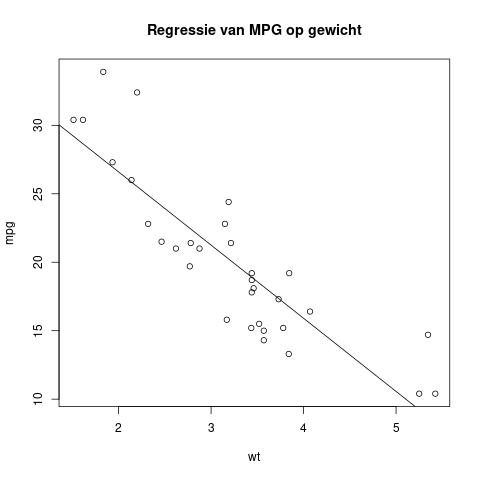
\includegraphics[scale=.5]{ren.jpeg}
\begin{lstlisting}[language=R]
    attach(mtcars)
    plot(wt, mpg)
    abline(lm(mpg~wt))
    title("Regression van MPG op Weight")
\end{lstlisting}


\chapter{Toepassingen}

wat moeten de leerlingen kunnen ?

\section{Voor het vak wiskunde}
\section{Voor OC}
\end{document}